\documentclass[a4paper,12pt,sffamily]{article}
\usepackage{datetime}
\usepackage{tikz}
\usepackage{algorithm}
\usepackage{amsmath}
\usepackage[noend]{algpseudocode}
\usepackage{fontspec}
\usepackage{minted}
\usemintedstyle[c]{tango}
\usepackage{listings}
\usetikzlibrary{trees}

\makeatletter
\def\BState{\State\hskip-\ALG@thistlm}
\makeatother

\begin{document}
\tikzstyle{every node}=[thick,anchor=west, rounded corners, font={\scriptsize\ttfamily}, inner sep=2.5pt]
\tikzstyle{selected}=[draw=blue,fill=blue!10]
\tikzstyle{root}=[selected, fill=blue!30]

\begin{titlepage}
  \begin{center}
    \vspace*{1cm}
    \Huge
    \textbf{Chapter 5}\\
    \vspace{0.5cm}
    \LARGE
    Traversing Directories
    \vfill
    \Large
    \textbf{Jonathan Reyna}\\
    College of Engineering and Computing\\
    Nova Southeastern University\\
    \usdate{\today}
  \end{center}
\end{titlepage}

\section{Problem Statement}
Exercise 5.8 requires a directory traversal implementation that uses both depth-first and breadth-first search algorithms. Chapter 5 discusses how to traverse directories with streams, using opendir and readdir. The solutions will use both of these POSIX functions to implement the algorithms.
\subsection{Algorithm: Depth-First Search}
The depth-first search portion of this problem suggests using a recursive algorithm. The algorithm is as follows:
\begin{algorithm}
  \caption{Depth-First Search}
  \label{depthfirst}
  \begin{algorithmic}[1]
    \Procedure{depthfirst}{}
    \For{each node at or below $root$}
    \State visit($node$)
    \If{$node$ is a directory}
    \State\Return{\Call{depthfirst}{$node$}}
    \EndIf
    \EndFor
    \EndProcedure
  \end{algorithmic}
\end{algorithm}\\
The algorithm implementation will traverse the following directory strucure:\\
\begin{tikzpicture}[%
    scale=.7,
    grow via three points={one child at (0.5,-0.65) and
    two children at (0.5,-0.65) and (0.5,-1.1)},
  edge from parent path={(\tikzparentnode.south) |- (\tikzchildnode.west)}]
  \node [root] {/}
    child {node [selected] {dirA}
      child {node {my1.dat}}
      child {node {my2.dat}}
      child {node [selected] {dirB}
        child {node {my1.dat}}
      }
    }
    child {node at (0,-3.5) [selected] {dirC}
      child {node {my3.dat}}
    };
\end{tikzpicture}
\subsection{Implementation}
The implementation uses an array to keep track of the files, as opposed to the directories, for the 
current function stack. Once the deepest directory has been reached, the array will be empied in reverse 
order. As the function stack unwinds, all files in the corresponding directory will be printed.
\renewcommand{\theFancyVerbLine}{
\sffamily\textcolor[rgb]{0.5,0.5,0.5}{\scriptsize\arabic{FancyVerbLine}}}

\begin{minted}[mathescape,
    linenos,
    numbersep=5pt,
    gobble=0,
    frame=lines,
  framesep=2mm]{c}

  /**
  * Cases:
  * 1. It's a file. Place it on the stack to be called 
  *    after the full depth has been reached.
  * 2. It's a directory (recursive case). Call self with 
  *    the directory path.
  */
  void depthfirst(const char *path) {

    DIR *dirp = NULL;

    if (path == NULL || strncmp(path, "", 1) == 0) {
      return;
      } else if ((dirp = opendir(path)) == NULL) {
      return;
    }

    char *regular_file_names[128];
    int regular_file_count = 0;
    char abs_path[256];

    struct dirent *dentp = NULL;
    while (dentp = readdir(dirp)) {

      if (strcmp(dentp->d_name, ".") == 0 || 
          strcmp(dentp->d_name, "..") == 0) {
        continue;
      }

      sprintf(abs_path, "%s/%s", path, dentp->d_name);

      if (dentp->d_type == DT_DIR) {
        printf("%s\n", abs_path);
        depthfirst(abs_path);
        } else {
        regular_file_names[regular_file_count] = 
          (char*)malloc(strlen(abs_path));
        strcpy(regular_file_names[regular_file_count++], 
               abs_path);
      }
    }
    for (--regular_file_count; 
         regular_file_count >= 0; 
         --regular_file_count) {
      printf("%s\n", regular_file_names[regular_file_count]);
      free(regular_file_names[regular_file_count]);
    }
    closedir(dirp);
  }
\end{minted}
\subsection{Environment}
The environment used for this implementation is Linux Mint.
\begin{minted}[numbersep=5pt,
	gobble=0,
	framesep=2mm]{bash}
meddling_monk at TRex in ~
$ lsb_release -a && uname -a
No LSB modules are available.
Distributor ID: LinuxMint
Description:    Linux Mint 17.2 Rafaela
Release:        17.2
Codename:       rafaela
Linux TRex 3.16.0-38-generic
#52~14.04.1-Ubuntu SMP Fri May 8 09:43:57 
UTC 2015 x86_64 x86_64 x86_64 GNU/Linux
\end{minted}
\subsection{Build}
\begin{figure}[H]
\centering
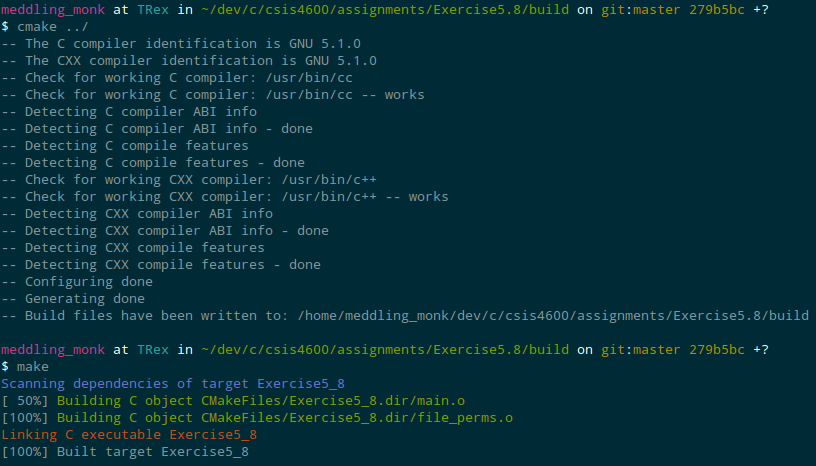
\includegraphics[width=1\linewidth]{./images/0}
\caption[build_1]{Build}
\label{fig:11}
\end{figure}
\subsection{Run}
For this run, GDB must be run with arguments pointing to the example directory, with the required 
directory strcuture.
\begin{figure}[H]
\centering
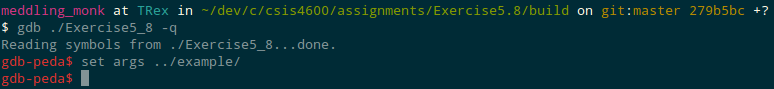
\includegraphics[width=1\linewidth]{./images/1}
\caption[GDB_prep]{Preparing GDB}
\label{fig:1}
\end{figure}
Once GDB has stepped into depthfirst(), the passed arguments can be verified.
\begin{figure}[H]
	\centering
	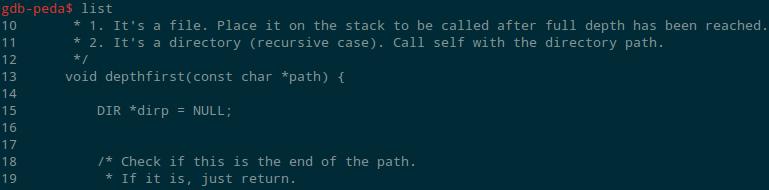
\includegraphics[width=1\linewidth]{./images/2}
	\caption[GDB_verify_1]{Verifying Function Scope}
	\label{fig:2}
\end{figure}
\begin{figure}[H]
	\centering
	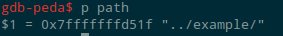
\includegraphics[width=.5\linewidth]{./images/3}
	\caption[GDB_verify_2]{Verifying function argument}
	\label{fig:3}
\end{figure}
The first check in \mintinline{c}{depthfirst()} ensures that the path parameter is not empty or 
\mintinline{c}{NULL}. If it is, \mintinline{c}{depthfirst()} returns. Otherwise, it establishes the 
directory stream with \mintinline{c}{opendir()}. \mintinline{c}{depthfirst()} also returns if 
\mintinline{c}{opendir()} does not assign a directory stream pointer to \mintinline{c}{dirp}. This 
establishes the error checks for \mintinline{c}{depthfirst()}, and satisfies the conditions required for 
this function to be recursive.
Since execution is beginning, and the directory tree structure has not been traversed, 
\mintinline{c}{opendir()} will succeed.
\begin{figure}[H]
	\centering
	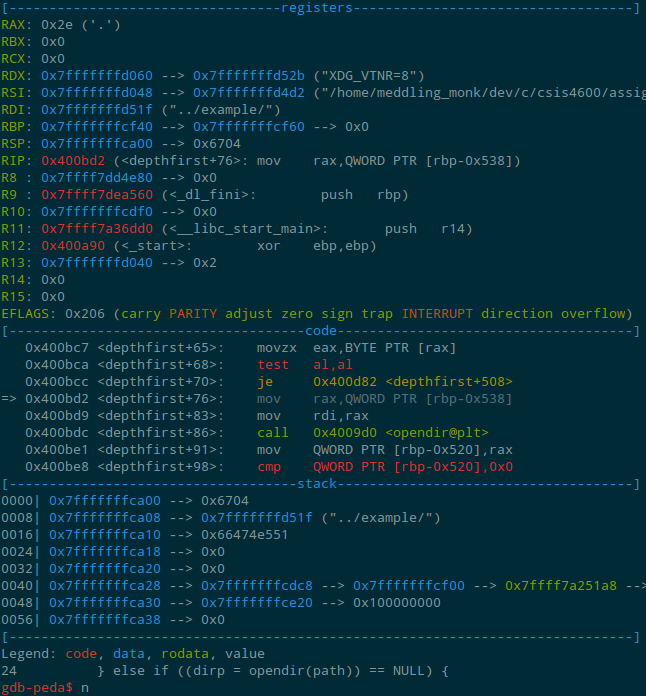
\includegraphics[width=1\linewidth]{./images/4}
	\caption[First_opendir]{First opendir() run}
	\label{fig:4}
\end{figure}
\mintinline{c}{dirp} was initialized on declaration to \mintinline{c}{NULL}, so memory allocation can be
verified by simply printing the pointer in GDB.
\begin{figure}[H]
	\centering
	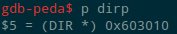
\includegraphics[width=.3\linewidth]{./images/5}
	\caption[print_dirp_pointer]{Printing dirp}
	\label{fig:5}
\end{figure}
Beginning the \mintinline{c}{while} loop, the result of \mintinline{c}{readdir(dirp)} is tested, as it
will be on each iteration.
\begin{figure}[H]
	\centering
	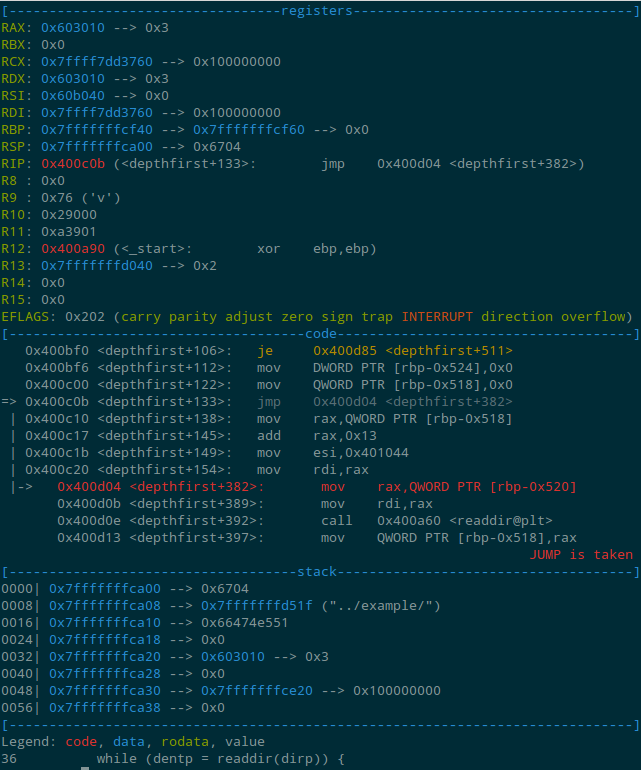
\includegraphics[width=1\linewidth]{./images/6}
	\caption[while_loop_test]{While loop test}
	\label{fig:6}
\end{figure}
The implementation must verify that \mintinline{c}{d_name} is not \mintinline{c}{"."} or 
\mintinline{c}{".."}, because visiting such nodes would cause extraneous entries to be printed. If this
iteration is not skipped, the next instruction will use \mintinline{c}{sprintf()} to store the absolute
path to the current entry. It is at this point, that the decision must be made whether or not to recurse.
\begin{figure}[H]
	\centering
	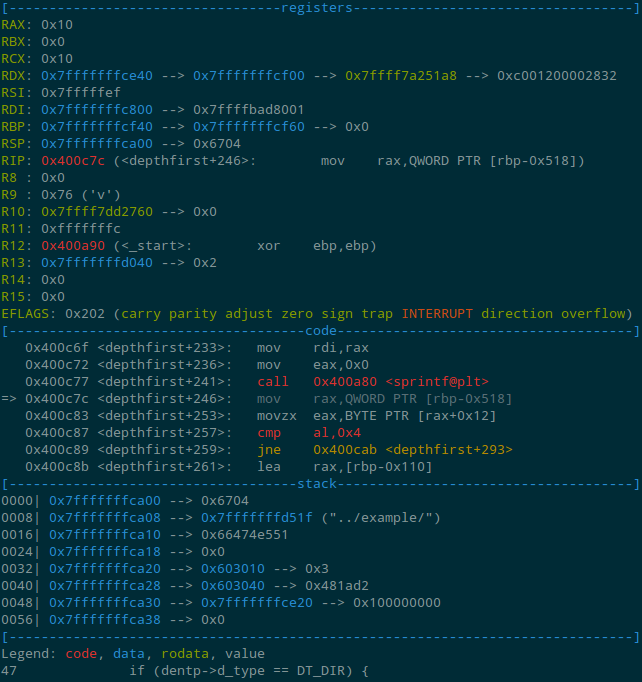
\includegraphics[width=1\linewidth]{./images/7}
	\caption[directory_check]{Check for recursive case}
	\label{fig:7}
\end{figure}
Using GDB, it is observed that this is indeed the recursive case, where \mintinline{c}{dentp->d_type} is
equivalent to \mintinline{c}{DT_DIR}, implying that the stream returned a directory on this iteration. As a result, this implementation will print the entry, and \mintinline{c}{depthfirst()} will be called
with the current directory as an argument.
\begin{figure}[H]
	\centering
	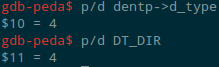
\includegraphics[width=.3\linewidth]{./images/8}
	\caption[verify_recursive_case]{Verifying recursive case}
	\label{fig:8}
\end{figure}
Stepping into the new \mintinline{c}{depthfirst()}, the registers, and stack, show references to 
\mintinline{bash}{dirA}.
\begin{figure}[H]
	\centering
	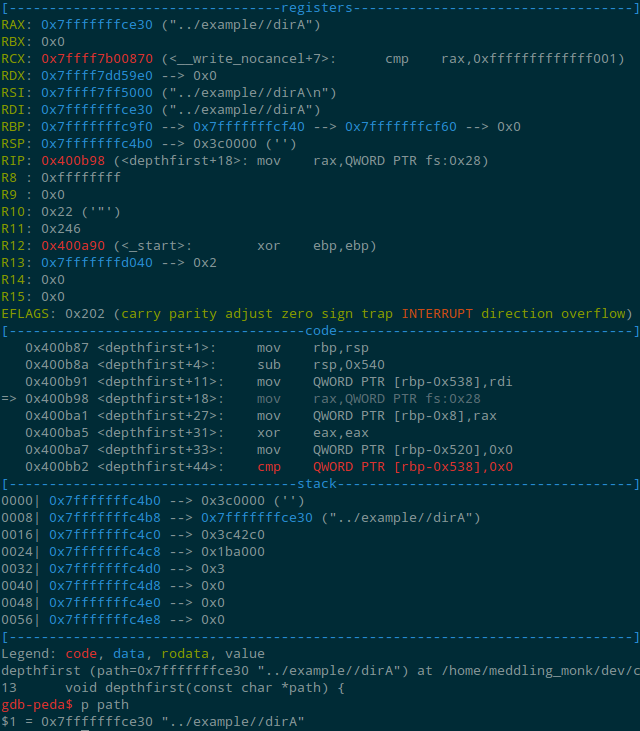
\includegraphics[width=1\linewidth]{./images/9}
	\caption[inside_first_recursive_case]{Inside first recursive case}
	\label{fig:9}
\end{figure}
The implementation will step through just as it did on the previous function stack. This time, however, the directory entry will be a file, not a directory.
\begin{figure}[H]
	\centering
	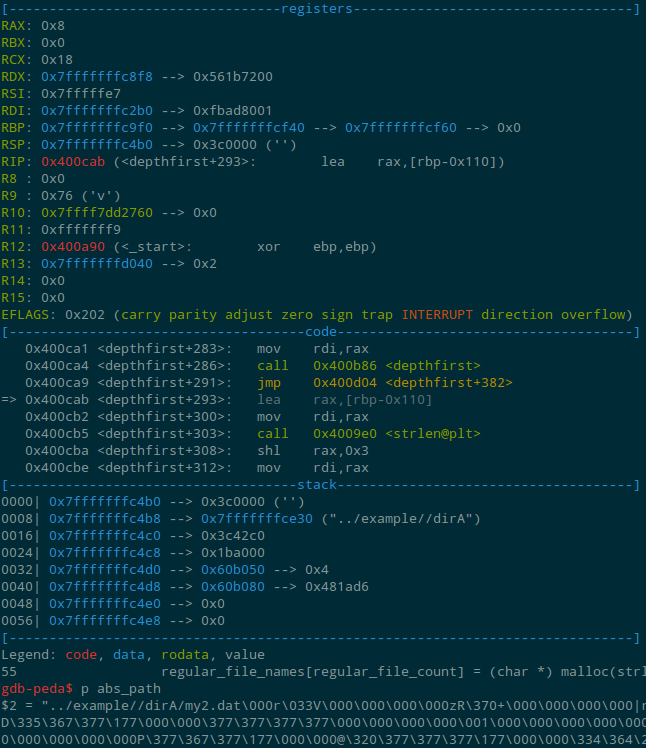
\includegraphics[width=1\linewidth]{./images/10}
	\caption[first_non_recursive_case]{First non-recursive case}
	\label{fig:10}
\end{figure}
As shown here, memory must be allocated to store the C-string in this element of the array. Once
allocated, \mintinline{c}{strcpy()} can be used to copy the C-string, representing the file, into the
array. The array element counter will also be incremented, so that later, those files can be printed
safely.
The next element in the stream is a directory, so that will be stepped over, since the recursive case 
has already been shown. Instead, the stepping will continue until the \mintinline{c}{while} block is 
finished, and the file array is printed.
\begin{figure}[H]
	\centering
	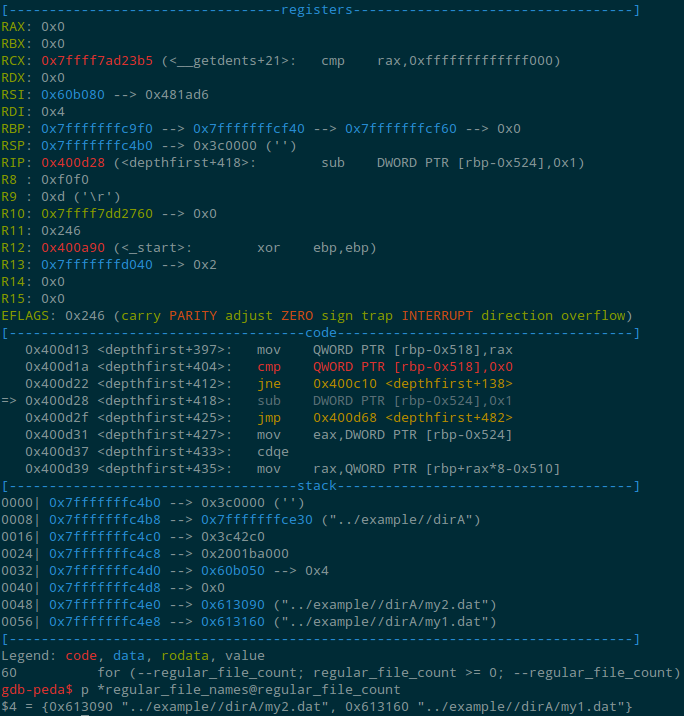
\includegraphics[width=1\linewidth]{./images/11}
	\caption[regular_file_loop_array]{Regular file loop and array}
	\label{fig:11}
\end{figure}
After these regular files are printed, the stack will unwind, and the regular files the parent 
directories will be printed. Once the root directory is reached, \mintinline{bash}{dirC} will be
recursed, and handled the same as \mintinline{bash}{dirA} was.
\end{document}

